\documentclass{scrreprt}
\usepackage{style}

\subject{4. Übung}
\title{389.055 Signale und Systeme 2 4.0}
\author{Byte Unit}
\uppertitleback{Unter GNU Free Document Lizenz}
\lowertitleback{\textcopyleft 2014 Byte Unit}
\date{\time}
%\publishers{}

\makeatletter
\AtBeginDocument{
    \hypersetup{
        pdftitle = {\@title},
        pdfsubject={\@subtitle},
        pdfauthor={\@author},
        pdfproducer={Latex (Debian/GNU Linux)},
        pdfkeywords={\@title, \@subject}
    }
}
\makeatother

\tikzstyle{point} = [draw, 
    fill=black,
    circle,
    inner sep=0pt]
\tikzstyle{block}=[rectangle,
    thick,
    minimum height=1cm,
    minimum width=1.5cm,
    draw=gray!80,
    fill=gray!20]    
\tikzstyle{sum} = [draw, 
    fill=gray!20,
    draw=gray!80,
    circle, 
    node distance=1cm]

\tikzstyle{input} = [coordinate]
\tikzstyle{output} = [coordinate]

\setcounter{tocdepth}{5}

\setcounter{chapter}{3}
\begin{document}
\chapter{Übung}
\begin{uebsp}
\begin{Exercise}
Das abgebildete System besteht aus zwei LTI–Systemen mit den Impulsantworten
$h_1[n]$ und $h_2[n]$. Berechnen Sie die Antwort $y[n]$ des Gesamtsystems auf
das Eingangssignal $x[n] = \delta[n] - \alpha \delta[n - 1], |\alpha| < 1$.
\begin{center}
\begin{tikzpicture}
    \matrix[row sep=0.5cm, column sep=0.5cm] {
        \node (input) {};&
        \node (h1) [block] {$h_1[n]$};&&
        \node (h2) [block] {$h_2[n]$};&
        \node (output) {};\\
        &\node (h1formula) {$h_1[n]=\left(\dfrac{1}{2}\right)^{|n|}\left(\sin\dfrac{\pi}{10}n\right)^2$}; &
        &\node (h2formula) {$h_2[n]=\alpha^n\sigma[n]$}; &\\
    };
    \draw [draw,->] (input) -- node[above] {$x[n]$} (h1);
    \draw [draw,->] (h1) -- (h2);
    \draw [draw,->] (h2) -- node[above] {$y[n]$} (output);
\end{tikzpicture}
\end{center}
\end{Exercise}
\begin{Answer}
    \begin{definition}[$\delta$-Einsimpuls]
        \[\delta[n]=\begin{cases}1 & n=0\\0 & n\neq 0\end{cases}\]
    \end{definition}
    \begin{definition}[$\sigma$-Sprungfunktion]
        \[\sigma[n]=\begin{cases}0 & \text{für }n<0\\1& \text{für }n\geq 0\end{cases}\]
    \end{definition}

    \begin{uebsp_theory}
        Das Ausgangssignal $y[n]$ eines linearen, zeitinvarianten Systems mit der Sprungantwort $h[n]$ und dem Eingangssignal $x[n]$ kann mit folgender Formel berechnet werden:
        \[y[n]=\sum_{k=-\infty}^\infty x[k]h[n-k]=\sum_{k=-\infty}^\infty x[n-k]h[k]\]
    \end{uebsp_theory}
    \begin{uebsp_theory}
        Ein System heißt BIBO(Bounded Input, Boundend Output)-Stabil, wenn gilt:
        \[\sum_{k=-\infty}^\infty\left|h[k]\right|<\infty\]
        $\Rightarrow$ Systeme mit endlich langer Impulsantwort sind immer stabil.
    \end{uebsp_theory}
    \begin{uebsp_theory}
        Bei der Kettenschaltung (Kaskadenschaltung (Reihenschaltung)) 2-er
        stabiler LTI-Systeme mit Impulsantworten $h_1[n]$ und $h_2[n]$ folgt:
        \[h[n]=\sum_{k=-\infty}^\infty h_1[k]h_2[n-k]=\sum_{k=-\infty}^\infty h_1[n-k]h_2[k]\]
        $\Rightarrow$ Es ist die Reihenfolge der Systeme egal:
        \begin{center}
        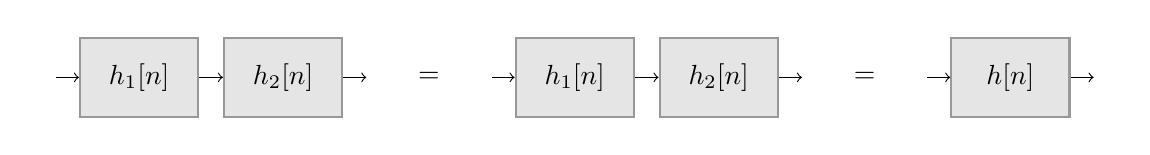
\begin{tikzpicture}
            \matrix[row sep=0.5cm, column sep=0.3cm] {
                \node (inputa) {};&
                \node (h1a) [block] {$h_1[n]$};&
                \node (h2a) [block] {$h_2[n]$};&
                \node (outputa) {};&
                \node (equa) {=};&
                \node (inputb) {};&
                \node (h1b) [block] {$h_1[n]$};&
                \node (h2b) [block] {$h_2[n]$};&
                \node (outputb) {};&
                \node (equa) {=};&
                \node (inputc) {};&
                \node (h) [block] {$h[n]$};&
                \node (outputc) {};\\
            };
            \draw [draw,->] (inputa) -- (h1a);
            \draw [draw,->] (h1a) -- (h2a);
            \draw [draw,->] (h2a) -- (outputa);
            \draw [draw,->] (inputb) -- (h1b);
            \draw [draw,->] (h1b) -- (h2b);
            \draw [draw,->] (h2b) -- (outputb);
            \draw [draw,->] (inputc) -- (h);
            \draw [draw,->] (h) -- (outputc);

        \end{tikzpicture}
        \end{center}
    \end{uebsp_theory}
    \begin{enumerate}[i)]
        \item Prüfen, ob alle Systeme BIBO-Systeme sind:
            \begin{eqnarray*}x[n] &=& \delta[n] - \alpha \delta[n - 1]\;\;\Rightarrow\;\;
                \sum_{k=-\infty}^\infty\left|\underbrace{\delta[k]}_{=1\text{ für }k=0} - \alpha \underbrace{\delta[k - 1]}_{=1\text{ für }k=1}\right|\;\;\;\fbox{\begin{minipage}{0.17\textwidth}$\Rightarrow$ mit $k=0$ bzw. $k=1\;\Rightarrow$ \end{minipage}}\\
                 &\Rightarrow& \left|1-\alpha\right|<\infty\;\;\forall|\alpha|<1\\
            h_1[n]&=&\left(\frac{1}{2}\right)^{|n|}\left(\sin\frac{\pi}{10}n\right)^2\;\;\Rightarrow\;\;
                \lim_{n\rightarrow\infty}h_1[n]=0\;\;\Rightarrow\;\;\\
                &\Rightarrow&\sum_{k=-\infty}^\infty\left|\left(\frac{1}{2}\right)^{|k|}\left(\sin\frac{\pi}{10}k\right)^2\right|<\infty\\
            h_2[n]&=&\alpha^n\sigma[n]\;\;\Rightarrow\;\;
                \lim_{n\rightarrow\infty}h_2[n]=0\;\;\Rightarrow\;\;
                \sum_{k=-\infty}^\infty\left|\alpha^n\sigma[n]\right|<\infty
            \end{eqnarray*}
        D.h. alle Systeme sind BIBO-Systeme.
        \item Umstellen der Reihenfolge auf folgende Form: (Ist möglich, da alles BIBO-Systeme sind)
            \begin{center}
            \begin{tikzpicture}
                \matrix[row sep=0.5cm, column sep=0.5cm] {
                    \node (input) {};&
                    \node (h2) [block] {$h_2[n]$};&
                    \node [above, red] {$y_1[n]$};&
                    \node (h1) [block] {$h_1[n]$};&
                    \node (output) {};\\
                    &\node (h2formula) {$h_2[n]=\alpha^n\sigma[n]$}; &
                    &\node (h1formula) {$h_1[n]=\left(\dfrac{1}{2}\right)^{|n|}\left(\sin\dfrac{\pi}{10}n\right)^2$}; &\\
                };
                \draw [draw,->] (input) -- node[above] {$x[n]$} (h2);
                \draw [draw,->] (h2) -- (h1);
                \draw [draw,->] (h1) -- node[above] {$y[n]$} (output);
            \end{tikzpicture}
            \end{center}
            \begin{uebsp_theory}
                Im folgenden muss oft die folgende (oder eine ähnliche) Gleichung gelöst werden:
                \[y[n]=\sum_{k=-\infty}^\infty\delta[k]x[n-k]\]
                Es ist ersichtlich, dass $\delta[k]$ nur an der Stelle $k=0$ den Wert $1$ annimmt, ansonsten ist sie immer $0$.

                Somit kann man das Summenzeichen vereinfachen, denn alle Summanden außer dem, bei dem $k=0$, sind 0.
                \[y[n]=\sum_{k=0}^0\delta[k]x[n-k]=\left.\delta[k]x[n-k]\right|_{k=0}=\underbrace{\delta[0]}_{=1}x[n-0]=x[n]\]
            \end{uebsp_theory}
        \item Berechnen von $y_1[n]$:
            \begin{eqnarray*}
                y_1[n] &=& \sum_{k=-\infty}^{\infty}\left(x[k]h_2[n-k]\right)=
                \sum_{k=-\infty}^{\infty}\left(\delta[k] - \alpha \delta[k - 1]\right)\alpha^{n-k}\sigma[n-k]\\
                y_1[n] &=& \sum_{k=-\infty}^{\infty}\underbrace{\delta[k]}_{=1\text{ für } k=0}\alpha^{n-k}\sigma[n-k] -\sum_{k=-\infty}^{\infty} \alpha \underbrace{\delta[k - 1]}_{=1\text{ für } k=1}\alpha^{n-k}\sigma[n-k]\\
                y_1[n] &=& \alpha^n\sigma[n]-\alpha\cdot\alpha^{n-1}\sigma[n-1] = \alpha^n\underbrace{(\sigma[n]-\sigma[n-1])}_{\delta[n]}=\alpha^n\cdot \underbrace{\delta[n]}_{=1\text{ für }n=0}\\
                y_1[n] &=& \alpha^0\cdot \delta[n] = \delta[n]
            \end{eqnarray*}
        \item Berechnen von $y[n]$:
            \begin{eqnarray*}
                y[n] &=& \sum_{k=-\infty}^{\infty}\left(y_1[k]h_1[n-k]\right)=
                \sum_{k=-\infty}^{\infty}\underbrace{\delta[k]}_{=1\text{ für }k=0}h_1[n-k]\;\;\;\fbox{$\Rightarrow$ mit $k=0$ folgt:}\\
                y[n] &=&h_1[n-0]=h_1[n]\\
            \end{eqnarray*}
    \end{enumerate}
\end{Answer}
\end{uebsp}

\begin{uebsp}
\begin{Exercise}
Berechnen Sie die Gesamtimpulsantwort $h[n]$ des abgebildeten Systems, das aus einzelnen
LTI–Systemen zusammengesetzt ist.
\begin{center}
\begin{tikzpicture}[auto, node distance=2cm,>=latex']
    \node [input, name=input] {};
    \node [block, right of=input] (h1){$h_1[n]$};
    \node [point, right=0.5cm of h1] (split){};
    \node [block, below right=0.25cm and 0.5cm of split] (h3) {$h_3[n]$};
    \node [right=0.5cm of h3] (h35){};
    \node [block, right=0.5cm of h35] (h4) {$h_4[n]$};
    \node [block, above=1cm of h35] (h2) {$h_2[n]$};
    \node [sum, right=5cm of split] (sum) {+};
    \node [output, right=3cm of sum] (output) {};

    \draw [draw,->] (input) -- node {$x[n]$} (h1);
    \draw [draw] (h1) -- (split);
    \draw [draw,->] (split) |- (h2.west);
    \draw [draw,->] (split) |- (h3);
    \draw [draw,->] (h3) -- (h4);
    \draw [draw,->] (h4) -| node[above left] {-} (sum);
    \draw [draw,->] (h2) -| (sum);
    \draw [draw,->] (sum) -- node {$y[n]=(x*h)[n]$} (output);
\end{tikzpicture}
\end{center}
Dabei sei:
\begin{eqnarray*}
    h_1[n]&=&\left(\frac{1}{2}\right)^n\sigma[n]\\
    h_2[n]&=&(n+1)\sigma[n]\\
    h_3[n]&=&h_2[n]\\
    h_4[n]&=&\delta[n-1]
\end{eqnarray*}
\end{Exercise}
\begin{Answer}
    \begin{definition}[$\delta$-Einsimpuls]
        \[\delta[n]=\begin{cases}1 & n=0\\0 & n\neq 0\end{cases}\]
    \end{definition}
    \begin{definition}[$\sigma$-Sprungfunktion]
        \[\sigma[n]=\begin{cases}0 & \text{für }n<0\\1& \text{für }n\geq 0\end{cases}\]
    \end{definition}
    \begin{uebsp_theory}
        Das Ausgangssignal $y[n]$ eines linearen, zeitinvarianten Systems mit der Sprungantwort $h[n]$ und dem Eingangssignal $x[n]$ kann mit folgender Formel berechnet werden:
        \[y[n]=\sum_{k=-\infty}^\infty x[k]h[n-k]=\sum_{k=-\infty}^\infty x[n-k]h[k]\]
    \end{uebsp_theory}
    \begin{uebsp_theory}
        Bei der Kettenschaltung (Kaskadenschaltung (Reihenschaltung)) 2-er 
        stabiler LTI-Systeme mit Impulsantworten $h_1[n]$ und $h_2[n]$ folgt:
        \[h[n]=\sum_{k=-\infty}^\infty h_1[k]h_2[n-k]=\sum_{k=-\infty}^\infty h_1[n-k]h_2[k]\]
        $\Rightarrow$ Es ist die Reihenfolge der Systeme egal:
        \begin{center}
        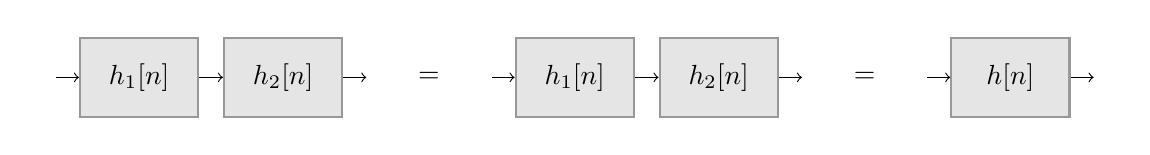
\begin{tikzpicture}
            \matrix[row sep=0.5cm, column sep=0.3cm] {
                \node (inputa) {};&
                \node (h1a) [block] {$h_1[n]$};&
                \node (h2a) [block] {$h_2[n]$};&
                \node (outputa) {};&
                \node (equa) {=};&
                \node (inputb) {};&
                \node (h1b) [block] {$h_1[n]$};&
                \node (h2b) [block] {$h_2[n]$};&
                \node (outputb) {};&
                \node (equa) {=};&
                \node (inputc) {};&
                \node (h) [block] {$h[n]$};&
                \node (outputc) {};\\
            };
            \draw [draw,->] (inputa) -- (h1a);
            \draw [draw,->] (h1a) -- (h2a);
            \draw [draw,->] (h2a) -- (outputa);
            \draw [draw,->] (inputb) -- (h1b);
            \draw [draw,->] (h1b) -- (h2b);
            \draw [draw,->] (h2b) -- (outputb);
            \draw [draw,->] (inputc) -- (h);
            \draw [draw,->] (h) -- (outputc);

        \end{tikzpicture}
        \end{center}
    \end{uebsp_theory}
    \begin{uebsp_theory}
        Bei der Paralellschaltung 2-er LTI-Systeme mit Impulsantworten 
        $h_1[n]$ und $h_2[n]$ folgt:
        \[h[n]=h_1[n]+h_2[n]\]
        \begin{center}
        \begin{tikzpicture}
            \node [input, name=inputa] {};
            \node [point, right=0.5cm of inputa] (split){};
            \node [block, below right=0.25cm and 0.5cm of split] (h1) {$h_1[n]$};
            \node [block, above=0.5cm of h1] (h2) {$h_2[n]$};
            \node [sum, right=2.2cm of split] (sum) {+};
            \node [output, right of=sum] (outputa) {};
            \node [right=1cm of outputa] (equ){=};
            \node [input, right=1cm of equ] (inputb){};
            \node [block, right=0.5cm of inputb] (h){h[n]};
            \node [output, right of=h] (outputb) {};

            \draw [draw,->] (inputa) -- (split);
            \draw [draw,->] (split) |- (h1);
            \draw [draw,->] (split) |- (h2);
            \draw [draw,->] (h2) -| (sum);
            \draw [draw,->] (h1) -| (sum);
            \draw [draw,->] (sum) -- (outputa);
            \draw [draw,->] (inputb) -- (h);
            \draw [draw,->] (h) -- (outputb);

        \end{tikzpicture}
        \end{center}
    \end{uebsp_theory}

    \textbf{TODO: wieso ist $h_3$ und $h_4$ stabil?}
    
    Am besten man zerlegt das gesamte System in kleine Teile:
    \begin{enumerate}[i)]
        \item Zusammenfassen und Berechnen der Serienschaltung von $h_3[n]$ und 
            $h_4[n]$ als $h_{34}[n]$:
            \begin{center}
            \begin{tikzpicture}[auto, node distance=2cm,>=latex']
                \node [input, name=input] {};
                \node [block, right=0.5cm of input] (h3) {$h_3[n]$};
                \node [block, right=0.5cm of h3] (h4) {$h_4[n]$};
                \node [output, right=0.5cm of h4] (output) {};

                \draw [draw,->] (input) -- (h3);
                \draw [draw,->] (h3) -- (h4);
                \draw [draw,->] (h4) -- (output);
            \end{tikzpicture}
            \end{center}
            Aus der Formel für die Reihenschaltung folgt:
        \begin{eqnarray*}
            h_{34}[n]&=&\sum_{k=-\infty}^\infty h_3[k]h_4[n-k]=
                \sum_{k=-\infty}^\infty (k+1)\sigma[k]\cdot
                \underbrace{\delta[n-k-1]}_{=1\text{ für }k=n-1}\\
                h_{34}[n]&=&(n\cancel-1\cancel+1)\sigma[n-1]=n\sigma[n-1]
        \end{eqnarray*}
        \item Zusammenfassen und Berechnen der Paralellschaltung von $h_2[n]$ und 
            $h_{34}[n]$ als $h_{2||34}[n]$:
            \begin{center}
            \begin{tikzpicture}
                \node [input, name=inputa] {};
                \node [point, right=0.5cm of inputa] (split){};
                \node [block, below right=0.25cm and 0.5cm of split] (h34)
                {$h_{34}[n]$};
                \node [block, above=0.5cm of h34] (h2) {$h_2[n]$};
                \node [sum, right=2.2cm of split] (sum) {+};
                \node [output, right of=sum] (outputa) {};

                \draw [draw,->] (inputa) -- (split);
                \draw [draw,->] (split) |- (h1);
                \draw [draw,->] (split) |- (h2);
                \draw [draw,->] (h2) -| (sum);
                \draw [draw,->] (h1) -|node[above left] {-} (sum);
                \draw [draw,->] (sum) -- (outputa);
            \end{tikzpicture}
            \end{center}
            Aus der Formel für die Reihenschaltung folgt:
        \begin{eqnarray*}
            h_{2||34}[n]&=&h_2[n]-h_{34}[n]=(n+1)\sigma[n]-n\sigma[n-1]=\underbrace{n\sigma[n]-n\sigma[n-1]}_{n\delta[n]}+\sigma[n]\\
            h_{2||34}[n]&=&n\delta[n]+\sigma[n]
        \end{eqnarray*}
        \item Zusammenfassen und Berechnen der Serienschaltung von $h_1[n]$ und 
            $h_{2||34}[n]$ als $h[n]$:
            \begin{center}
            \begin{tikzpicture}[auto, node distance=2cm,>=latex']
                \node [input, name=input] {};
                \node [block, right=0.5cm of input] (h1) {$h_{1}[n]$};
                \node [block, right=0.5cm of h1] (h234) {$h_{2||34}[n]$};
                \node [output, right=0.5cm of h234] (output) {};

                \draw [draw,->] (input) -- (h1);
                \draw [draw,->] (h1) -- (h234);
                \draw [draw,->] (h234) -- (output);
            \end{tikzpicture}
            \end{center}
            \begin{definition}[Geometrische Reihe]
                \[\sum_{n=0}^\infty a^n=\frac{1}{1-a}\;\;\forall
                    |a|<1\;\;\;\;\text{ und }\;\;\;\;
                    \sum_{n=0}^{N-1} a^n=\begin{cases}N&a=1\\
                        \frac{1-a^N}{1-a}&\text{sonst }\forall N\geq0\end{cases}\]
            \end{definition}
            \begin{eqnarray*}
                h[n]&=&\sum_{k=-\infty}^\infty h_1[k]h_{2||34}[n-k]=
                \sum_{k=-\infty}^\infty \left(\frac{1}{2}\right)^k\sigma[k]
                ((n-k)\delta[n-k]+\sigma[n-k])\\
                h[n]&=&\sum_{k=-\infty}^\infty \left(\frac{1}{2}\right)^k\sigma[k]
                (n-k)\underbrace{\delta[n-k]}_{=1\text{ für
                }k=n}+\sum_{k=-\infty}^\infty
                \left(\frac{1}{2}\right)^k\sigma[k]\sigma[n-k]\\
                h[n]&=&\left(\frac{1}{2}\right)^n\sigma[n]\underbrace{(n-n)}_{=0}+\sum_{k=-\infty}^\infty
                \left(\frac{1}{2}\right)^k\underbrace{\sigma[k]}_{=1\text{ für
                }k\geq0\;\;}\underbrace{\sigma[n-k]}_{\;\;=1\text{ für }n\geq
            k}\fbox{\begin{minipage}{0.2\linewidth}Somit geht $\sum$ von
            $k=0$ bis $n$\end{minipage}}\\
            h[n]&=&\underbrace{\sum_{k=0}^n\left(\frac{1}{2}\right)^k}_{\text{Geom.
            Reihe}}=\frac{1-\left(\frac{1}{2}\right)^{n+1}}{1-\frac{1}{2}}=
            \frac{1-\left(\frac{1}{2}\right)^{n+1}}{\frac{1}{2}}=
            2-\cancel2\left(\frac{1}{2}\right)^{n\cancel{+1}}\\
            h[n]&=&2-\left(\frac{1}{2}\right)^n\;\;\;\forall
            n\geq0\;\;\;\Rightarrow\;\;\;h[n]=\left(2-\left(\frac{1}{2}\right)^n\right)\sigma[n]
            \end{eqnarray*}
        \end{enumerate}
    \end{Answer}
\end{uebsp}

\begin{uebsp}
\begin{Exercise}
Gegeben ist ein LTI–System mit der Impulsantwort
\[h[n]=12\left(\left(-\frac{1}{3}\right)^n-\left(-\frac{1}{2}\right)^n\right)\sigma[n].\]
\begin{enumerate}[a)]
    \item Berechnen und skizzieren Sie die Sprungantwort $a[n]$ des Systems.
    \item Zur Vermeidung von Überschwingen der Sprungantwort $a[n]$ wird nun zum gegebenen System ein System in Kette geschaltet. 
        Dieses Entzerrersystem wird durch die folgende Eingangs/Ausgangsbeziehung beschrieben:
        \[y[n]=ax[n]+bx[n-1]+cx[n-2].\]
        \begin{center}
            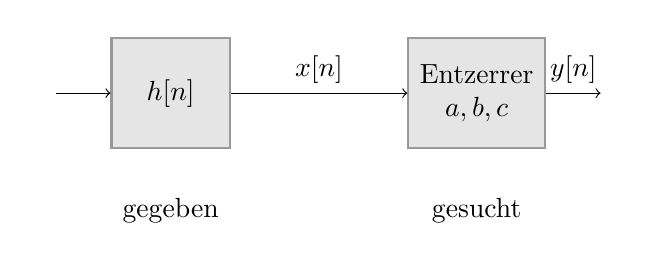
\begin{tikzpicture}
                \matrix[row sep=0.5cm, column sep=0.7cm] {
                    \node (input) {};&
                    \node (h) [block,minimum height=1.4cm] {$h[n]$};&
                    \node [above] {$x[n]$};&
                    \node (e) [block,minimum height=1.4cm]
                    {\begin{minipage}{1.5cm}\begin{center}Entzerrer\\$a,b,c$\end{center}\end{minipage}};&
                    \node (output) {};\\
                    &\node (hdesc) {gegeben}; &
                    &\node (edesc) {gesucht}; &\\
                };
                \draw [draw,->] (input) -- (h);
                \draw [draw,->] (h) -- (e);
                \draw [draw,->] (e) -- node[above] {$y[n]$} (output);
            \end{tikzpicture}
            \end{center}
        Wie sind die Koeffizienten $a$, $b$, $c$ zu wählen, so dass das
        Gesamtsystem kein Überschwingen zeigt, d.h. die Sprungantwort des
        entzerrten Gesamtsystems ist $\tilde a[n]=\sigma[n-n_0]$?

    \item Wie groß sollte zweckmäßigerweise die Zeitverzögerung $n_0$ gewählt
    werden?
\end{enumerate}
\end{Exercise}
\begin{Answer}
\begin{enumerate}[a)]
    \item Berechnen und skizzieren Sie die Sprungantwort $a[n]$ des Systems:
    \begin{uebsp_theory}
        Das Ausgangssignal $y[n]$ eines linearen, zeitinvarianten Systems mit der Sprungantwort $h[n]$ und dem Eingangssignal $x[n]$ kann mit folgender Formel berechnet werden:
        \begin{equation}
            y[n]=\sum_{k=-\infty}^\infty x[k]h[n-k]=\sum_{k=-\infty}^\infty
            x[n-k]h[k]
            \label{eq:ausgang_eingang}
        \end{equation}
    \end{uebsp_theory}
    \begin{uebsp_theory}
        Ist das Eingangssignal eines Systems mit der Sprungantwort $h[n]$ die 
        Sprungfunktion $\sigma[n]$, dann erhält man am Ausgang die Sprungantwort:

        (Eingesetzt für $x[n]=\sigma[n]$ in \fref{eq:ausgang_eingang} erhält man somit)
        \[a[n]=\sum_{k=-\infty}^\infty \sigma[k]h[n-k]=\sum_{k=-\infty}^\infty
        \sigma[n-k]h[k]\]
    \end{uebsp_theory}
    \begin{definition}[Geometrische Reihe]
        \[\sum_{n=0}^\infty a^n=\frac{1}{1-a}\;\;\forall
            |a|<1\;\;\;\;\text{ und }\;\;\;\;
            \sum_{n=0}^{N-1} a^n=\begin{cases}N&a=1\\
                \frac{1-a^N}{1-a}&\text{sonst }\forall N\geq0\end{cases}\]
    \end{definition}
    \begin{eqnarray*}
        a[n]&=&\sum_{k=-\infty}^\infty\sigma[n-k]h[k]=
            \sum_{k=-\infty}^\infty\sigma[n-k]12\left(\left(-\frac{1}{3}\right)^k-\left(-\frac{1}{2}\right)^k\right)\sigma[k]\\
        a[n]&=&12\left(\sum_{k=-\infty}^\infty\underbrace{\sigma[k]}_{=1\text{
            für }k\geq0\;}\underbrace{\sigma[n-k]}_{\;=1\text{ für }n\geq
            k}\left(\left(-\frac{1}{3}\right)^k-\left(-\frac{1}{2}\right)^k\right)\right)
            \fbox{\begin{minipage}{0.2\linewidth}Somit
                geht $\sum$ von $k=0$ bis $n$\end{minipage}}\\
        a[n]&=&12\left(\underbrace{\sum_{k=0}^n\left(-\frac{1}{3}\right)^k}_{Geom. Reihe}
            -\underbrace{\sum_{k=0}^n\left(-\frac{1}{2}\right)^k}_{Geom. Reihe}\right)\\
        a[n]&=&12\left(\frac{1-\left(-\frac{1}{3}\right)^{n+1}}{1+\frac{1}{3}}
            -\frac{1-\left(-\frac{1}{2}\right)^{n+1}}{1+\frac{1}{2}}\right)\;\;\;\forall
            n\geq0\;\Rightarrow\fbox{Mit $\sigma[n]$ multiplizieren}\\
        a[n]&=&12\left(\frac{1-\left(-\frac{1}{3}\right)^{n+1}}{\frac{4}{3}}
            -\frac{1-\left(-\frac{1}{2}\right)^{n+1}}{\frac{3}{2}}\right)\sigma[n]\\
        a[n]&=&12\left(\frac{3}{4}\left(1-\left(-\frac{1}{3}\right)^{n+1}\right)
            -\frac{2}{3}\left(1-\left(-\frac{1}{2}\right)^{n+1}\right)\right)\sigma[n]\\
        a[n]&=&\cancel{12}\left(\frac{9\left(1-\left(-\frac{1}{3}\right)^{n+1}\right)
            -8\left(1-\left(-\frac{1}{2}\right)^{n+1}\right)}{\cancel{12}}\right)\sigma[n]\\
        a[n]&=&\left(1-9\left(-\frac{1}{3}\right)^{n+1}
            +8\left(-\frac{1}{2}\right)^{n+1}\right)\sigma[n]\\
        a[n]&=&\left(1-\cancel9\left(-\frac{1}{3}\right)^{n-1}\frac{1}{\cancel9}
            +\cancel8\left(-\frac{1}{2}\right)^{n-2}\left(-\frac{1}{\cancel8}\right)\right)\sigma[n]\\
        a[n]&=&\left(1-\left(-\frac{1}{3}\right)^{n-1}
            -\left(-\frac{1}{2}\right)^{n-2}\right)\sigma[n]
    \end{eqnarray*}
        \def\lbl{$a[n]=(1-\left(-\frac{1}{3}\right)^{n-1}
            -\left(-\frac{1}{2}\right)^{n-2})\sigma[n]$}
        \begin{center}
            \begin{tikzpicture}
                \begin{axis}[%
                    big,
                    legend style={at={(1,1.12), anchor=north west}},
                    xlabel={$n$},
                    ylabel={$y[n]$}]
                    \addplot+[domain=-4:-1,ycomb,black,thick,mark=*,samples=4]
                    {0};
                    \addlegendentry[align=left]{\lbl};
                    \addplot+[domain=0:15,ycomb,black,thick,mark=*,forget
                        plot,samples=16] {1-(-1/3)^(x-1)-(-1/2)^(x-2)};
                \end{axis}
            \end{tikzpicture}
        \end{center}
        \item Berechnen der Koeffizienten $a$, $b$, $c$, um Überschwingen zu
        vermeiden ($\tilde a[n]=\sigma[n-n_0]$)
        {\footnotesize
        \begin{eqnarray*}
            y[n]&=&\tilde a[n]=\sigma[n-n_0]=ax[n]+bx[n-1]+cx[n-2]\\
            \sigma[n-n_0]&=&a\left(1-\left(-\frac{1}{3}\right)^{n-1}-\left(-\frac{1}{2}\right)^{n-2}\right)\sigma[n]
                +b\left(1-\left(-\frac{1}{3}\right)^{n-2}-\left(-\frac{1}{2}\right)^{n-3}\right)\sigma[n-1]\\
                &&\;\;+c\left(1-\left(-\frac{1}{3}\right)^{n-3}-\left(-\frac{1}{2}\right)^{n-4}\right)\sigma[n-2]
        \end{eqnarray*}}
        Das Promblem sind nun die lästigen $\sigma$-Sprünge, die Zu den
        Zeitpunkten $n=0,1,2$ und $n_0$ auftreten. 

        Wenn wir jedoch ein sehr großes $n$ betrachten ($n>n_0$ und $n>2$), dann
        muss logischerweise die Gleichung noch genauso gelten, jedoch haben wir
        den Vorteil, dass wir uns das $\sigma$ wegdenken können, denn es
        besitzen bereits alle $\sigma$-Sprünge den Wert $1$.

        Somit gilt $\forall n>n_0$ und $\forall n>2$ folgendes:
        \begin{eqnarray*}
            1&=&a\left(1-\left(-\frac{1}{3}\right)^{n-1}-\left(-\frac{1}{2}\right)^{n-2}\right)\cdot 1
                +b\left(1-\left(-\frac{1}{3}\right)^{n-2}-\left(-\frac{1}{2}\right)^{n-3}\right)\cdot 1\\
                &&\;\;+c\left(1-\left(-\frac{1}{3}\right)^{n-3}-\left(-\frac{1}{2}\right)^{n-4}\right)\cdot
                1\\
            1&=&a+b+c-a\left(-\frac{1}{3}\right)^{n-3}\frac{1}{3^2}-b\left(-\frac{1}{3}\right)^{n-3}\left(-\frac{1}{3}\right)-c\left(-\frac{1}{3}\right)^{n-3}\\
            &&\;\;-a\left(-\frac{1}{2}\right)^{n-4}\frac{1}{2^2}-b\left(-\frac{1}{2}\right)^{n-4}\left(-\frac{1}{2}\right)-c\left(-\frac{1}{2}\right)^{n-4}\\
            1&=&a+b+c-\left(\frac{a}{9}-\frac{b}{3}+c\right)\left(-\frac{1}{3}\right)^{n-3}
                -\left(\frac{a}{4}-\frac{b}{2}+c\right)\left(-\frac{1}{2}\right)^{n-4}
        \end{eqnarray*}
        Nun können wir mittels Koeffizientenvergleich die Werte für $a$, $b$ und
        $c$ bestimmen (das geht allerdings nur, weil
        $\left(-\frac{1}{3}\right)^{n-3}$ und $\left(-\frac{1}{2}\right)^{n-4}$
        linear unabhängig sind)
        \begin{enumerate}[i)]
            \item $\begin{aligned}[t]1=a+b+c\end{aligned}$
            \item $\begin{aligned}[t]0=\left(\frac{a}{9}-\frac{b}{3}+c\right)\left(-\frac{1}{3}\right)^{n-3}\;\;\Rightarrow\;\;
                0=\left(\frac{a}{9}-\frac{b}{3}+c\right)\;\;\Rightarrow\;\;
                b=3\left(\frac{a}{9}+c\right)\end{aligned}$
            \item
            $\begin{aligned}[t]0=\left(\frac{a}{4}-\frac{b}{2}+c\right)\left(-\frac{1}{2}\right)^{n-4}\;\;\Rightarrow\;\;
                0=\left(\frac{a}{4}-\frac{b}{2}+c\right)\;\;\Rightarrow\;\;
                b=2\left(\frac{a}{4}+c\right)\end{aligned}$
        \end{enumerate}
        Somit erhalten wir:
        \[
            2\left(\frac{a}{4}+c\right)=3\left(\frac{a}{9}+c\right)\;\;\Rightarrow\;\;
            \frac{a}{2}+2c=\frac{a}{3}+3c\;\Rightarrow\;
            \frac{3a}{6}-\frac{2a}{3}=c\;\Rightarrow\;
            \frac{a}{6}=c\;\Rightarrow\;a=6c
        \]
        Somit können wir $c$ berechnen:
        \[1=a+\underbrace{b}_{\frac{a}{2}+2c}+c=a+\underbrace{\frac{a}{2}}_{3c}+2c+c=6c+3c+3c=12c\;\;\Rightarrow\;\;c=\frac{1}{12}\]
        Somit können wir $a$ berechnen:
        \[a=6c=\frac{6}{12}=\frac{1}{2}\]
        Somit können wir $b$ berechnen:
        \[b=\frac{a}{2}+2c=\frac{1}{4}+\frac{2}{12}=\frac{5}{12}\]

        Somit erhalten wir als neue Gleichung:
        \begin{eqnarray}
            \sigma[n-n_0]&=&\frac{1}{2}\left(1-\left(-\frac{1}{3}\right)^{n-1}-\left(-\frac{1}{2}\right)^{n-2}\right)\cdot
            \sigma[n]\\
                &&\;\;+\frac{5}{12}\left(1-\left(-\frac{1}{3}\right)^{n-2}-\left(-\frac{1}{2}\right)^{n-3}\right)\cdot
                \sigma[n-1]\\
                &&\;\;+\frac{1}{12}\left(1-\left(-\frac{1}{3}\right)^{n-3}-\left(-\frac{1}{2}\right)^{n-4}\right)\cdot
                \sigma[n-2]
            \label{eq:komponenten}
        \end{eqnarray}

        \item Gesucht ist nun die Zeitverzögerung $n_0$:
            Durch $\sigma[n], \sigma[n-1]$ und $\sigma[n-2]$ folgt, dass
            $n_0\geq 0$ sein muss.
            Wenn wir uns nun die Komponenten in \fref{eq:komponenten} ansehen:\\
            $\begin{aligned}[t]A=\frac{1}{2}\left(1-\left(-\frac{1}{3}\right)^{n-1}-\left(-\frac{1}{2}\right)^{n-2}\right)\cdot
                \sigma[n]\end{aligned}$\\
            $\begin{aligned}[t]B=\frac{5}{12}\left(1-\left(-\frac{1}{3}\right)^{n-2}-\left(-\frac{1}{2}\right)^{n-3}\right)\cdot
                \sigma[n-1]\end{aligned}$\\
            $\begin{aligned}[t]C=\frac{1}{12}\left(1-\left(-\frac{1}{3}\right)^{n-3}-\left(-\frac{1}{2}\right)^{n-4}\right)\cdot
                \sigma[n-2]\end{aligned}$\\
           Dann können wir uns die ersten paar Werte berechnen:
           \begin{center}
           \begin{tabular}{c|cccccc}
            n&  $0$&  $1$    &$2$    &$3$  &$4$ &$\cdots$\\
            \hline
            A&$0$&$1$&$\frac{1}{6}$&$\frac{25}{36}$&$\frac{85}{216}$&$\cdots$\\
            B&$0$&$0$&$\frac{5}{6}$&$\frac{5}{36}$&$\frac{125}{216}$&$\cdots$\\
            C&$0$&$0$&$0$&$\frac{6}{36}$&$\frac{6}{216}$&$\cdots$\\
            \hline
            $\sum$&$0$&$1$&$1$&$1$&$1$&$\cdots$\\
           \end{tabular}
           \end{center}
           Somit sieht man gut, dass $\sum=(A+B+C)$ ab $n\geq1$ immer $1$ ergibt.
           
           Folglich muss $n_0=1$ sein.

        \begin{center}
            \begin{tikzpicture}
                \def\lbl{$\sigma[n-n_0]=\sigma[n-1]$}

                \begin{axis}[%
                    big,
                    legend style={at={(1,1.12), anchor=north west}},
                    xlabel={$n$},
                    ylabel={$y[n]$}]
                    \addplot+[domain=-4:0,ycomb,black,thick,mark=*,samples=5]
                    {0};
                    \addlegendentry[align=left]{\lbl};
                    \addplot+[domain=1:10,ycomb,black,thick,mark=*,samples=10]
                    {1};
                \end{axis}
            \end{tikzpicture}
        \end{center}

        \textbf{TODO: Wie kommt man darauf, dass der Entzerrer aus 3 Komponenten
        besteht? Kann er auch aus 2 oder 1ner Komponente bestehen?}
    \end{enumerate}
\end{Answer}
\end{uebsp}

\begin{uebsp}
\begin{Exercise}
Ein System sei als Kettenschaltung zweier Teilsysteme realisiert. Das erste
Teilsystem ist durch die Eingangs/Ausgangsbeziehung
\[z[n]=\sum_{k=n-N+1}^nx[k]=\sum_{k=-\infty}^\infty h_1[n-k]x[k]\]
charakterisiert. Vom zweiten System ist die Impulsantwort bekannt:
\[h_2[n]=2\sin\frac{\pi}{N}\sin\frac{2\pi n}{N}\sigma[n]\]

\begin{center}
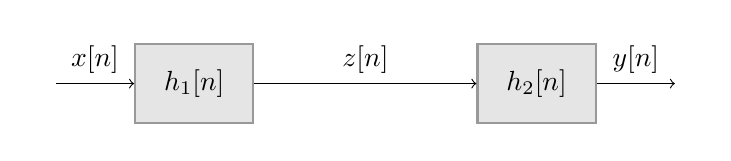
\begin{tikzpicture}
    \matrix[row sep=0.5cm, column sep=1cm] {
        \node (input) {};&
        \node (h1) [block] {$h_1[n]$};&
        \node [above] {$z[n]$};&
        \node (h2) [block] {$h_2[n]$};&
        \node (output) {};\\
    };
    \draw [draw,->] (input) -- node[above] {$x[n]$} (h1);
    \draw [draw,->] (h1) -- (h2);
    \draw [draw,->] (h2) -- node[above] {$y[n]$} (output);
\end{tikzpicture}
\end{center}

\begin{enumerate}[a)]
    \item Berechnen und skizzieren Sie:
        \begin{enumerate}
            \item die Impulsantwort $h_1[n]$ des ersten Teilsystems,
            \item die Impulsantwort $h[n]$ des Gesamtsystems,
        \end{enumerate}
    \item Berechnen Sie die Antwort $y[n]$ des Gesamtsystems auf das
    Eingangssignal $x[n] = \sin\frac{2\pi n}{N}, -\infty < n < \infty$.
    \item Vertauschen Sie jetzt die Reihenfolge der beiden Teilsysteme und
    wiederholen Sie Punkt b: Warum erhält man dabei ein anderes Ergebnis, 
    obwohl doch beide Teilsysteme LTI–Systeme sind und die Faltungsoperation 
    normalerweise assoziativ ist?
\end{enumerate}
\end{Exercise}
\begin{Answer}
\begin{enumerate}[a)]
    \item Berechnen und skizzieren Sie:\\
        \begin{enumerate}
            \item die Impulsantwort $h_1[n]$ des ersten Teilsystems,
                \begin{eqnarray*}
                    z[n]&=&\sum_{k=n-N+1}^n x[k]\\
                \end{eqnarray*}
                Will man aus einer Summe mit Grenzen eine unendliche Summe erzeugen, die
                mit den Sprungfunktionen $\sigma$ arbeitet, berechnet man anhand der
                Grenzen der Summe die Argumente der $\sigma$-Funktion:

                Die untere Grenze lautet: $k=n-N+1$, d.h. wir brauchen folgende
                Funktion: 
                \[f[k]=\begin{cases}1&k\geq n-N+1\\0&\text{
                    sonst}\end{cases}\;\;\Rightarrow\;\;\sigma[k-n+N-1]\]

                Die obere Grenze lautet: $k=n$, d.h. wir brauchen folgende
                Funktion:
                \[f[k]=\begin{cases}1&k\leq n\\0&\text{
                    sonst}\end{cases}\;\;\Rightarrow\;\;\sigma[-k+n]\]

                $k-n$ das Argument der $\sigma$-Funktion:
                $\sigma[k-n]$.

                Anschließend müssen wir nur noch beide Grenzen miteinander
                multiplizieren:

                \begin{eqnarray*}
                    z[n]&=&\sum_{k=n-N+1}^nx[k]=
                        \sum_{k=-\infty}^\infty(\sigma[n-k]\cdot\sigma[-n+N-1+k])x[k]\\
                \end{eqnarray*}

                \begin{uebsp_theory}
                    Wird am Eingang der Dirac-Impuls $\delta[n]$ angelegt,
                    erhält man am Ausgang die Impulsantwort $h[n]$.
                \end{uebsp_theory}

                Um die Impulsantwort zu berechnen, ersetzen wir in der
                Eingangs-/Ausgangsbeziehung das $x[n]$ durch $\delta[n]$:
                \begin{eqnarray*}
                    h_1[n]&=&\sum_{k=-\infty}^\infty(\sigma[-n+N-1+k]\cdot\sigma[n-k])
                        \underbrace{\delta[k]}_{=1\text{ für }k=0}\\
                    h_1[n]&=&\sigma[-n+N-1]\cdot \sigma[n]
                \end{eqnarray*}
                Somit brauchen wir eine Fallunterscheidung: Dazu zerlegen wir
                die Funktion $h_1$:

                $\sigma[n]=1\text{ für }n\geq0$ und \\
                $\sigma[-n+N-1]=1\text{ für }n\leq N-1$.\\
                Somit gilt:
                \[h_1[n]=\begin{cases}1&\forall (n)\in [0,N-1]\\0&\text{sonst}\end{cases}\]
                Und wir können $h_1[n]$ auch schreiben, als
                \[h_1[n]=\sigma[n]-\sigma[n-(N-1)]=\sigma[n]-\sigma[n-N+1]\]
            \item die Impulsantwort $h[n]$ des Gesamtsystems,
                \begin{uebsp_theory}
                    Bei der Kettenschaltung (Kaskadenschaltung (Reihenschaltung)) 2-er 
                    stabiler LTI-Systeme mit Impulsantworten $h_1[n]$ und $h_2[n]$ folgt:
                    \[h[n]=\sum_{k=-\infty}^\infty h_1[k]h_2[n-k]=\sum_{k=-\infty}^\infty h_1[n-k]h_2[k]\]
                    $\Rightarrow$ Es ist die Reihenfolge der Systeme egal:
                    \begin{center}
                    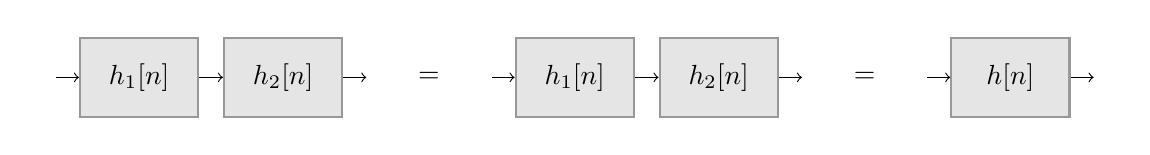
\begin{tikzpicture}
                        \matrix[row sep=0.5cm, column sep=0.3cm] {
                            \node (inputa) {};&
                            \node (h1a) [block] {$h_1[n]$};&
                            \node (h2a) [block] {$h_2[n]$};&
                            \node (outputa) {};&
                            \node (equa) {=};&
                            \node (inputb) {};&
                            \node (h1b) [block] {$h_1[n]$};&
                            \node (h2b) [block] {$h_2[n]$};&
                            \node (outputb) {};&
                            \node (equa) {=};&
                            \node (inputc) {};&
                            \node (h) [block] {$h[n]$};&
                            \node (outputc) {};\\
                        };
                        \draw [draw,->] (inputa) -- (h1a);
                        \draw [draw,->] (h1a) -- (h2a);
                        \draw [draw,->] (h2a) -- (outputa);
                        \draw [draw,->] (inputb) -- (h1b);
                        \draw [draw,->] (h1b) -- (h2b);
                        \draw [draw,->] (h2b) -- (outputb);
                        \draw [draw,->] (inputc) -- (h);
                        \draw [draw,->] (h) -- (outputc);

                    \end{tikzpicture}
                \end{center}
                \end{uebsp_theory}
                Somit können wir die Impulsantwort des Gesamtsystems wie folgt
                berechnen:
                \begin{eqnarray*}
                    h[n]&=&\sum_{k=-\infty}^\infty h_1[k]h_2[n-k] = \sum_{k=-\infty}^\infty h_1[n-k]h_2[k]\\
                    h[n]&=&\sum_{k=-\infty}^\infty
                        (\sigma[n-k]-\sigma[n-k-N+1])2\sin\frac{\pi}{N}\sin\frac{2\pi
                        k}{N}\sigma[k]\\
                    h[n]&=&\sum_{k=-\infty}^\infty
                        2\sin\frac{\pi}{N}\sin\frac{2\pi
                        k}{N}(\sigma[n-k]-\sigma[n-k-N+1])\underbrace{\sigma[k]}_{=1\text{
                        für }k\geq 0}\\
                        &\Rightarrow&\fbox{Somit ist ersichtlich, dass $h[n]=0$ für
                            $k<0$}\\
                    h[n]&=&\sum_{k=0}^\infty
                        2\sin\frac{\pi}{N}\sin\frac{2\pi
                        k}{N}(\sigma[n-k]-\sigma[n-k-N+1])\underbrace{\cancel{\sigma[k]}}_{=1\text{
                        für }k\geq 0}\\
                    h[n]&=&\sum_{k=0}^\infty
                        2\sin\frac{\pi}{N}\sin\frac{2\pi
                        k}{N}\underbrace{\sigma[n-k]}_{=1\text{ für }k\leq n}-\sum_{k=0}^\infty
                        2\sin\frac{\pi}{N}\sin\frac{2\pi
                        k}{N}\underbrace{\sigma[n-k-N+1]}_{=1\text{ für }k\leq
                        n-N+1}\\
                    h[n]&=&\sum_{k=0}^n
                        2\sin\frac{\pi}{N}\sin\frac{2\pi
                        k}{N}
                        -\sum_{k=0}^{n-N+1}
                        2\sin\frac{\pi}{N}\sin\frac{2\pi
                        k}{N}\\
                        h[n]&=&2\sin\frac{\pi}{N}\left(\sum_{k=0}^n
                        \sin\frac{2\pi
                        k}{N}
                        -\sum_{k=0}^{n-N+1}
                        \sin\frac{2\pi
                        k}{N}\right)
                \end{eqnarray*}
                \begin{definition}[Eulersche Formel]
                    \[e^{j\,\varphi} = \cos\left(\varphi
                    \right) + j\,\sin\left( \varphi\right).\]
                    Außerdem gilt:
                    \[\sin x=\frac{e^{jx}-e^{-jx}}{2j}\;\;\text{ bzw.
                    }\;\;\cos x=\frac{e^{jx}+e^{-jx}}{2}\]
                \end{definition}
                Wir ziehen nun beide Summen aus der Gleichung raus: 
                \[\sum_{k=0}^n\sin\frac{2\pi k}{N}=
                    \sum_{k=0}^n\frac{e^{j\frac{2\pi k}{N}}-e^{-j\frac{2\pi k}{N}}}{2j}=
                    \frac{1}{2j}\left(\sum_{k=0}^n
                e^{j\frac{2\pi k}{N}}-\sum_{k=0}^ne^{-j\frac{2\pi k}{N}}\right)\]
                \[\sum_{k=0}^{n-N+1}\sin\frac{2\pi k}{N}=
                    \sum_{k=0}^{n-N+1}\frac{e^{j\frac{2\pi k}{N}}-e^{-j\frac{2\pi k}{N}}}{2j}=
                    \frac{1}{2j}\left(\sum_{k=0}^{n-N+1}
                e^{j\frac{2\pi k}{N}}-\sum_{k=0}^{n-N+1}e^{-j\frac{2\pi k}{N}}\right)\]
                \begin{definition}[Geometrische Reihe]
                    \[\sum_{n=0}^\infty a^n=\frac{1}{1-a}\;\;\forall
                        |a|<1\;\;\;\;\text{ und }\;\;\;\;
                        \sum_{n=0}^{N-1} a^n=\begin{cases}N&a=1\\
                            \frac{1-a^N}{1-a}&\text{sonst }\forall N\geq0\end{cases}\]
                \end{definition}
                Mit der Geometrischen Reihe erhalten wir:
                \begin{eqnarray*}
                    \sum_{k=0}^n\sin\frac{2\pi k}{N}&=&\frac{1}{2j}\left(\sum_{k=0}^n
                    e^{j\frac{2\pi k}{N}}-\sum_{k=0}^ne^{-j\frac{2\pi
                    k}{N}}\right)=
                    \frac{1}{2j}\left(\sum_{k=0}^{j\frac{2\pi n}{N}}
                    e^{k}-\sum_{k=0}^{-j\frac{2\pi n}{N}}e^k\right)\\
                    &=&\frac{1}{2j}\left(\frac{1-e^{j\frac{2\pi
                    (n+1)}{N}}}{1-e^{j\frac{2\pi
                    (1)}{N}}}-\frac{1-e^{-j\frac{2\pi
                    (n+1)}{N}}}{1-e^{-j\frac{2\pi
                    (1)}{N}}}\right)
                \end{eqnarray*}
                \begin{eqnarray*}\sum_{k=0}^{n-N+1}\sin\frac{2\pi k}{N}&=&
                    \frac{1}{2j}\left(\sum_{k=0}^{n-N+1}
                    e^{j\frac{2\pi k}{N}}-\sum_{k=0}^{n-N+1}e^{-j\frac{2\pi
                    k}{N}}\right)\\
                    &=&\frac{1}{2j}\left(\sum_{k=0}^{j\frac{2\pi (n-N+1)}{N}}
                    e^{k}-\sum_{k=0}^{-j\frac{2\pi (n-N+1)}{N}}e^k\right)\\
                    &=&\frac{1}{2j}\left(\sum_{k=0}^{j\frac{2\pi (n-N+1)}{N}}
                    e^{k}-\sum_{k=0}^{-j\frac{2\pi (n-N+1)}{N}}e^k\right)\\
                    &=&\frac{1}{2j}\left(\frac{1-e^{j\frac{2\pi
                    (n+2)}{N}}}{1-e^{j\frac{2\pi
                    (1)}{N}}}-\frac{1-e^{-j\frac{2\pi
                    (n+2)}{N}}}{1-e^{-j\frac{2\pi
                    (1)}{N}}}\right)
                \end{eqnarray*}

                \begin{eqnarray*}
                        h[n]&=&2\sin\frac{\pi}{N}\left(\sum_{k=0}^n
                        \sin\frac{2\pi
                        k}{N}
                        -\sum_{k=0}^{n-N+1}
                        \sin\frac{2\pi
                        k}{N}\right)\\
                        h[n]&=&2\sin\frac{\pi}{N}\left(
                        \frac{1}{2j}\left(\frac{1-e^{j\frac{2\pi
                            (n+1)}{N}}}{1-e^{j\frac{2\pi
                            (1)}{N}}}-\frac{1-e^{-j\frac{2\pi
                            (n+1)}{N}}}{1-e^{-j\frac{2\pi
                            (1)}{N}}}\right)
                        -\frac{1}{2j}\left(\frac{1-e^{j\frac{2\pi
                            (n+2)}{N}}}{1-e^{j\frac{2\pi
                            (1)}{N}}}-\frac{1-e^{-j\frac{2\pi
                            (n+2)}{N}}}{1-e^{-j\frac{2\pi
                            (1)}{N}}}\right)\right)\\
                            &\Rightarrow&\fbox{Mit \href{http://www.wolframalpha.com/input/?i=simplify+\%28\%281-e^\%28i+2+pi+\%28n\%2B1\%29\%2FN\%29\%29\%2F\%281-e^\%28i+2+pi\%2FN\%29\%29-\%281-e^\%28-\%28i2+pi+\%28n\%2B1\%29\%2FN\%29\%29\%29\%2F\%281-e^\%28-\%28i+2+pi\%2FN\%29\%29\%29\%29}{Wolfram Alpha}
                            folgt:}\\
                            h[n]&=&2\sin\frac{\pi}{N}\left(\frac{1}{\cancel{2j}}
                            \left(\cancel{2j}\csc\left(\frac{\pi}{N}\right)\sin
                                \left(\frac{\pi
                                n}{N}\right)\sin\left(\frac{\pi(n+1)}{N}\right)\right)-
                                \frac{1}{\cancel{2j}}
                                \left(\cancel{2j}\csc\left(\frac{\pi}{N}\right)\sin
                                \left(\frac{\pi
                                (n+1)}{N}\right)\sin\left(\frac{\pi(n+2)}{N}\right)\right)\right)\\
                            h[n]&=&2\sin\frac{\pi}{N}\left(
                                \left(\csc\left(\frac{\pi}{N}\right)\sin
                                \left(\frac{\pi
                                n}{N}\right)\sin\left(\frac{\pi(n+1)}{N}\right)\right)-
                                \left(\csc\left(\frac{\pi}{N}\right)\sin
                                \left(\frac{\pi
                                (n+1)}{N}\right)\sin\left(\frac{\pi(n+2)}{N}\right)\right)\right)\\
                            &\Rightarrow&\fbox{Mit $\csc(x)=\frac{1}{sin(x)}$
                            folgt:}\\
                            h[n]&=&2\cancel{\sin\frac{\pi}{N}}\left(
                                \left(\frac{1}{\cancel{sin\left(\frac{\pi}{N}\right)}}\sin
                                \left(\frac{\pi
                                n}{N}\right)\sin\left(\frac{\pi(n+1)}{N}\right)\right)-
                                \left(\frac{1}{\cancel{sin\left(\frac{\pi}{N}\right)}}\sin
                                \left(\frac{\pi
                                (n+1)}{N}\right)\sin\left(\frac{\pi(n+2)}{N}\right)\right)\right)\\
                            h[n]&=&2\left(
                                \left(\sin
                                \left(\frac{\pi
                                n}{N}\right)\sin\left(\frac{\pi(n+1)}{N}\right)\right)-
                                \left(\sin
                                \left(\frac{\pi
                                (n+1)}{N}\right)\sin\left(\frac{\pi(n+2)}{N}\right)\right)\right)\\
                \end{eqnarray*}
                %here helps wa out: simplify ((1-e^(i 2 pi (n+1)/N))/(1-e^(i 2 pi/N))-(1-e^(-(i2 pi (n+1)/N)))/(1-e^(-(i 2 pi/N))))
        \end{enumerate}
    \item Berechnen Sie die Antwort $y[n]$ des Gesamtsystems auf das
    Eingangssignal $x[n] = \sin\frac{2\pi n}{N}, -\infty < n < \infty$.
    \item Vertauschen Sie jetzt die Reihenfolge der beiden Teilsysteme und
    wiederholen Sie Punkt b: Warum erhält man dabei ein anderes Ergebnis, 
    obwohl doch beide Teilsysteme LTI–Systeme sind und die Faltungsoperation 
    normalerweise assoziativ ist?
\end{enumerate}
\end{Answer}
\end{uebsp}

\begin{uebsp}
\begin{Exercise}
Sie sollen ein zeitdiskretes System untersuchen, von dem die Beziehung zwischen
Eingangssignal $x[n]$ und Ausgangssignal $y[n]$ gegeben ist:
\[y[n]=\sum_{k=n-1}^{n+1}(x[k+1]-x[k]+x[k-1])\]
\begin{enumerate}[a)]
    \item Prüfen Sie (mit Beweis), ob das System die folgenden Eigenschaften besitzt:
        \begin{enumerate}[1)]
            \item Linearität,
            \item Kausalität,
            \item Stabilität,
            \item Zeitinvarianz.
        \end{enumerate}
    \item Berechnen und skizzieren Sie die Impulsantwort und die Übertragungsfunktion 
        des Systems.
    \item Welches Ausgangssignal liefert das System für $x[n] = (-1)^n\;\;\forall n$?
    \item Nun wird das System mit dem Signal $x[n] = \lambda^n$ angeregt.
        Wie ist $\lambda$ zu wählen, damit $y[n] \equiv 0$ ist?
    \item Geben Sie eine Realisierung des Systems an.
\end{enumerate}
\end{Exercise}
\begin{Answer}
    Als erstes werde ich die Formel für $y[n]$ etwas vereinfachen:
    \begin{eqnarray*}
        y[n]&=&\sum_{k=n-1}^{n+1}(x[k+1]-x[k]+x[k-1]\\
        y[n]&=&x[n-1+1]-\cancel{x[n-1]}+x[n-1-1]+\cancel{x[n+1]}-x[n]+\cancel{x[n-1]}\\
            &&\;\;+x[n+1+1]-\cancel{x[n+1]}+x[n+1-1]\\
        y[n]&=&x[n]+x[n-2]-\cancel{x[n]}+x[n+2]+\cancel{x[n]}\\
        y[n]&=&x[n-2]+x[n]+x[n+2]\\
    \end{eqnarray*}
    \begin{uebsp_theory}
        Ein zeitdiskretes System verarbeitet das Eingangssignal $x[n]$ durch
        Anwendung eines zeitdiskret arbeitenden Algorithmus
        $\mathcal{T}\{\cdot\}$ zu einem Ausgangssignal $y[n]$.
        \begin{center}
        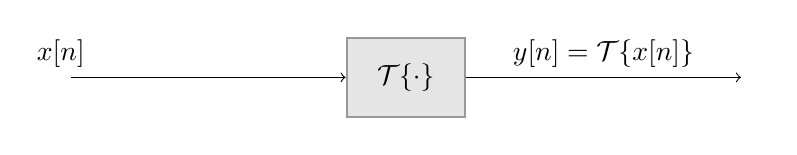
\begin{tikzpicture}
            \matrix[row sep=0.5cm, column sep=3.5cm] {
                \node (input) {};&
                \node (T) [block] {$\mathcal{T}\{\cdot\}$};&
                \node (output) {};\\
            };
            \draw [draw,->] (input) node[above] {$x[n]$} -- (T);
            \draw [draw,->] (T) -- node[above] {$y[n]=\mathcal{T}\{x[n]\}$} (output);
        \end{tikzpicture}
        \end{center}
    \end{uebsp_theory}
    \begin{enumerate}[a)]
        \item Prüfen Sie (mit Beweis), ob das System die folgenden Eigenschaften besitzt:

            Generell gilt lt. Tutor: sobald die Impulsantwort berechenbar ist,
            handelt es sich um ein LTI-System, somit sind die 2 Bedingungen
            Linearität und Zeitinvarianz immer erfüllt, wenn die Impulsantwort
            berechenbar ist. (siehe \fref{item:impulsantwort})
            \begin{enumerate}[1)]
                \item Linearität,
                    \begin{definition}[Linearität(Superpositionsprinzip)]:\\
                        Bei einem linearen System ist die Antwort auf eine Summe
                        von Eingangssignalen gleich der Summe der
                        Einzelantworten:
                        \[y[n]=\mathcal{T}\left\{\sum_ia_ix_i[n]\right\}
                            =\sum_ia_i\mathcal{T}\left\{x_i[n]\right\}
                        =\sum_ia_iy_i[n]\]
                        \[x[n]=\sum_i a_ix_i[n]\;\;\Rightarrow\;\;y[n]=\sum_ia_iy_i[n]\]
                        Zusätzlich besitzen lin. Systeme noch folgende
                        Eigenschaft:
                        \[x[n]\equiv0\;\;\Rightarrow\;\;y[n]\equiv0\]
                    \end{definition}
                    Wir ersetzen einfach überall $x[n]$ durch $\sum_ia_ix_i[n]$:
                \begin{eqnarray*}
                    y[n]&=&x[n-2]+x[n]+x[n+2]\;\;\Rightarrow\;\;\fbox{setze $x[n]=\sum_ia_ix_i[n]$}\\
                    y[n]&=&\sum_ia_ix_i[n-2]+\sum_ia_ix_i[n]+\sum_ia_ix_i[n+2]\\
                    y[n]&=&\sum_ia_i\underbrace{(x_i[n-2]+x_i[n]+x_i[n+2])}_{y_i[n]}\\
                    y[n]&=&\sum_ia_i{y_i[n]}\;\;\Rightarrow\;\;\fbox{linear}
                \end{eqnarray*}
                Da $y[n]=\sum_ia_i{y_i[n]}$ das Ergebnis ist, das rauskommen
                muss, wenn es sich um ein lineares System handelt, muss es
                folglich linear sein.
                \item Kausalität,
                    \begin{definition}[Kausalität]:\\
                        Bei kausalen Systemen eilt die Systemantwort der
                        Systemanregung nicht vorraus. Die Systemantwort hängt
                        nur von den vergangenen Eingangssignalwerten ab.
                        \[h[n]=0\;\;\forall\;\;n<0\]
                        Wobei $h[n]$ die Impulsantwort darstellt.
                    \end{definition}
                    Da die Impulsantwort folgende ist: (Berechnung und Plot, siehe \fref{item:impulsantwort})
                    \[h[n]=\delta[n-2]+\delta[n]+\delta[n+2]\]
                    Ist leicht ersichtlich, dass $h[n]\neq0$ für $n<0$:
                    z.B: Einschalten zum Zeitpunkt $n$, dann müsste gelten: $h[n]=0\;\;\forall n<0$.
                    Das ist aber nicht erfüllt, siehe Plot.$\;\Rightarrow\;$\fbox{Akausal}
                \item Stabilität,
                    \begin{definition}[Stabilität]:\\
                        Ein System heißt stabil, wenn es auf ein
                        amplitudenbegrenztes Eingangssignal mit einem
                        amplitudenbegrenzten Ausgangssignal antwortet.
                        (BIBO...Bounded Input - Bounded Output)

                        Für zeitdiskrete LTI-Systeme gilt:
                        \[\sum_{k=-\infty}^\infty\left|h[k]\right|<\infty\]
                        $\Rightarrow$ Systeme mit endlich langer Impulsantwort sind immer stabil.

                        Wobei $h[n]$ die Impulsantwort darstellt.
                    \end{definition}
                    Da die Impulsantwort folgende ist: (Berechnung und Plot, siehe \fref{item:impulsantwort})
                    \[h[n]=\delta[n-2]+\delta[n]+\delta[n+2]\]
                    folgt:
                    \[\sum_{k=-\infty}^\infty |h[k]|=\sum_{k=-\infty}^\infty\underbrace{\delta[k-2]}_{=1\text{ für }k=2}+\underbrace{\delta[k]}_{=1\text{ für }k=0}+\underbrace{\delta[k+2]}_{=1\text{ für }k=-2}=3<\infty\;\Rightarrow\;\fbox{BIBO-stab.}\]
                \item Zeitinvarianz.
                    \begin{definition}[Zeitinvarianz]:\\
                        Bei zeitinvarianten Systemen ändert sich die Form des
                        Ausgangssignals nicht, wenn das Eingangssignal zu
                        verschiedenen Zeitpunkten angelegt wird. (Es tritt nur
                        eine Zeitverschiebung auf)
                        \[\mathcal{T}\{\delta[n-k]\}=h[n-k]\]
                        \[\mathcal{T}\{x[n-k]\}=y[n-k]\]
                    \end{definition}
                Im folgenden werden wir zuerst $x[n]$ durch $x[n-k]$ ersetzen, 
                dann werden wir dieses $x[n-k]$ in die Formel von $y[n]$
                anstatt dem $x[n]$ einsetzen.

                Als nächstes müssen wir in der Formel von $y[n]$ das $n$ durch
                $n-k$ ersetzen und mit dem obigen Ergebnis vergleichen.
                 \begin{eqnarray*}
                     \mathcal{T}\{x[n-k]\}&=&x[n-k-2]+x[n-k]+x[n-k+2]\\
                    y[n-k]&=&x[n-k-2]+x[n-k]+x[n-k+2]\\
                    &\Rightarrow&\mathcal{T}\{x[n-k]\}=y[n-k]\;\;\Rightarrow\;\;\fbox{zeitinvariant,
                 da beide gleich.}
                \end{eqnarray*}                   
            \end{enumerate}
        \item Berechnen und skizzieren der Impulsantwort und der
            Übertragungsfunktion:
            \label{item:impulsantwort}
            \begin{uebsp_theory}
                Wird am Eingang der Der Dirac-Impuls $\delta[n]$ angelegt,
                erhält man am Ausgang die Impulsantwort $h[n]$.
            \end{uebsp_theory}
            Um die Impulsantwort zu berechnen, ersetzen wir in der bereits
            vereinfachten Formel das Eingangssignal $x[n]$ durch den Impuls 
            $\delta[n]$:
            \[y[n]=x[n-2]+x[n]+x[n+2]\;\;\Rightarrow\;\;
                h[n]=\delta[n-2]+\delta[n]+\delta[n+2]\]
            \begin{center}
                \begin{tikzpicture}
                    \begin{axis}[%
                        big,
                        legend style={at={(1,1.12), anchor=north west}},
                        xlabel={$n$},
                        ylabel={$h[n]$}]
                        \addplot+[domain=-4:-1,ycomb,black,thick,mark=*,samples=4]
                        {0};
                        \addlegendentry[align=left]{$h[n]=\delta[n-2]+\delta[n]+\delta[n+2]$};
                        \addplot+[ycomb,black,thick,mark=*,forget plot,samples
                            at={-2,0,2}] {1};
                        \addplot+[ycomb,black,thick,mark=*,forget plot,samples
                            at={-6,...,-3,-1,1,3,4,...,6}] {0};
                    \end{axis}
                \end{tikzpicture}
            \end{center}
            Nun wenden wir uns der Übertragungsfunktion zu:
            \begin{uebsp_theory}
                Die Übertragungsfunktion $H(e^{j\theta})$ ist die
                Fouriertransformierte der Impulsantwort:
                \[H(e^{j\theta})=\sum_{k=-\infty}^\infty h[k]e^{-j\theta
                k}=\mathcal{FT}\{h[n]\}\]
            \end{uebsp_theory}
            Wir setzen somit die vorher berechnete Impulsantwort $h[n]$ in die
            Summe ein:
            \begin{eqnarray*}
                H(e^{j\theta})&=&\sum_{k=-\infty}^\infty h[k]e^{-j\theta k}\\
                H(e^{j\theta})&=&\sum_{k=-\infty}^\infty\left(
                    \underbrace{\delta[n-2]}_{=1\text{ für
                    }k=2}+\underbrace{\delta[n]}_{=1\text{ für
                    }k=0}+\underbrace{\delta[n+2]}_{=1\text{ für
                    }k=-2}\right)e^{-j\theta k}\\
                H(e^{j\theta})&=&e^{-j\theta -2} + \underbrace{e^{-j\theta
                    0}}_{=1} + e^{-j\theta
                    2} = e^{-j\theta 2} + 1 + e^{j\theta 2}
            \end{eqnarray*}
            \begin{definition}[Eulersche Formel]
                \[e^{j\varphi}=\cos(\varphi)+j\cdot\sin(\varphi)\]
            \end{definition}
            Mit der eulerschen Formel folgt:
            \begin{eqnarray*}
                H(e^{j\theta})&=&e^{-j\theta 2} + 1 + e^{j\theta 2}=
                    1+\underbrace{\cos(-\theta 2)}_{=\cos(\theta 2)}
                    +j\underbrace{\sin(-\theta 2)}_{=-\sin(\theta 2)}
                    +\cos(\theta 2)+j\sin(\theta 2)\\
                H(e^{j\theta})&=&
                    1+\cos(\theta 2)-\cancel{j\sin(\theta 2)}+\cos(\theta
                    2)+\cancel{j\sin(\theta 2)}=1+2\cos(\theta 2)
            \end{eqnarray*}
            \begin{center}
                \begin{tikzpicture}
                    \begin{axis}[%
                        big,
                        legend style={at={(1,1.12), anchor=north west}},
                        xtick={-6.2831, -3.1416, 0, 3.1416, 6.2831},
                        xticklabels={$-2\pi$,$-\pi$,$0$,$\pi$,$2\pi$},
                        xlabel={$n$},
                        ylabel={$h[n]$}]
                    \addplot[domain=-3*pi:3*pi, samples=101] {1+2*cos(deg(x))}; 
                    \legend{$1+2\cos(\theta 2)$}
                    \end{axis}
                \end{tikzpicture}
            \end{center}
        \item Welches Ausgangssignal liefert das System für $x[n] = (-1)^n\;\;\forall n$?
            Einsetzen von $(-1)^n$ für $x[n]$ in die vereinfachte Formel:
            \[y[n]=x[n-2]+x[n]+x[n+2]=(-1)^{n-2}+(-1)^n+(-1)^{n+2}\]
            Man kann $(-1)^{n}$ auch als cos darstellen: $\cos(n\pi)=(-1)^n$

            Mit dem cos kann man zeigen, dass gilt: 
            \[\cos((n+2z)\pi)=\cos(n\pi)\;\;\Rightarrow\;\;(-1)^{n+2z}=(-1)^{n}\;\;\;\;\forall n\in\mathbb{N},\;z\in\mathbb{Z}\]
            Da gilt: $(-1)^{n+2z}=(-1)^{n}\;\;\forall n\in\mathbb{N},\;\;z\in\mathbb{Z}$ folgt:
            \[y[n]=(-1)^{n-2}+(-1)^n+(-1)^{n+2}=(-1)^{n}+(-1)^n+(-1)^{n}=3\cdot (-1)^n\]
 
     \item Nun wird das System mit dem Signal $x[n] = \lambda^n$ angeregt.
        Wie ist $\lambda$ zu wählen, damit $y[n] \equiv 0$ ist?
             Einsetzen von $\lambda^n$ für $x[n]$ in die vereinfachte Formel:
            \begin{eqnarray*}
                y[n]&=&x[n-2]+x[n]+x[n+2]=\lambda^{n-2}+\lambda^n+\lambda^{n+2}=0\\
                0&=&\lambda^n(\lambda^{-2}+\lambda^0+\lambda^{2})\;\;\Rightarrow\;\;0=\lambda^{-2}+\lambda^0+\lambda^{2}\;\;\fbox{Multiplizieren mit: $\lambda^2$}\\
                0&=&\lambda^{0}+\lambda^2+\lambda^{4}\;\;\fbox{Subst.: $\lambda^{2x}=\alpha^{x}$}\\
                0&=&\alpha^{0}+\alpha^1+\alpha^{2}=1+\alpha+\alpha^2
            \end{eqnarray*}
            \begin{definition}[Quadratische Lösungsformel]
                \[x_{1,2}=\frac{-b\pm\sqrt{b^2-4ac}}{2a}\]
            \end{definition}
            Eingesetzt in Quadratische Lösungsformel:
            \begin{eqnarray*}
                \alpha_{1,2}&=&\frac{-1\pm\sqrt{1^2-4\cdot1\cdot1}}{2\cdot1}=\frac{-1\pm\sqrt{1-4}}{2}=\frac{-1\pm\sqrt{-3}}{2}=\frac{-1}{2}\pm\sqrt{\frac{-3}{4}}\\
                \alpha_{1,2}&=&\frac{-1}{2}\pm j\frac{\sqrt3}{2}\;\;\fbox{Rücksubst: $\alpha^{x}=\lambda^{\frac{x}{2}}=\sqrt{\lambda^x}$}\\
                \lambda_{1,2,3,4}&=&\sqrt{\frac{-1}{2}\pm j\frac{\sqrt3}{2}}\\
            \end{eqnarray*}
        \item Geben Sie eine Realisierung des Systems an.
            Hier haben wir ein Problem: ein reales System kann nur kausal sein, wir haben hier aber ein akausales System: $\Rightarrow$ $h[n]$ muss um 2 Zeiteinheiten verzögert werden und wir erhalten als neue Gleichung:
            \[y[n]=x[n]+x[n-2]+x[n-4]\]
         \begin{center}
        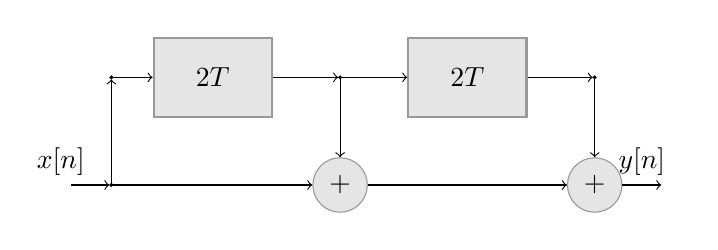
\begin{tikzpicture}
            \matrix[row sep=0.5cm, column sep=0.5cm] {
                &\node (splita) [point]{};&
                \node (2Ta) [block] {$2T$};&
                \node (splitb) [point]{};&
                \node (2Tb) [block] {$2T$};&
                \node (splitc) [point]{};&\\
                \node (input) {};&
                \node (splitd) [point]{};&&
                \node (suma) [sum] {$+$};&&
                \node (sumb) [sum] {$+$};&
                \node (output) {};\\
            };
            \draw [draw,->] (input)node[above] {$x[n]$} -- (splitd);
            \draw [draw,->] (splita) -- (2Ta);
            \draw [draw,->] (2Ta) -- (splitb);
            \draw [draw,->] (splitb) -- (2Tb);
            \draw [draw,->] (2Tb) -- (splitc);
            \draw [draw,->] (splitd) -- (splita);
            \draw [draw,->] (splitd) -- (suma);
            \draw [draw,->] (suma) -- (sumb);
            \draw [draw,->] (splitb) -- (suma);
            \draw [draw,->] (splitc) -- (sumb);
            \draw [draw,->] (sumb) --node[above] {$y[n]$} (output);
        \end{tikzpicture}
        \end{center}
   
    \end{enumerate}
\end{Answer}
\end{uebsp}

\end{document}
